\documentclass{ctexart}
\usepackage{graphicx}
\usepackage{cite}
\usepackage{amsmath,amssymb,amsfonts}
\usepackage{algorithmic}
\usepackage{listings}
\usepackage{textcomp}
\usepackage{hyperref} 
\usepackage{caption}
\usepackage{subfigure}
\usepackage{graphicx,xcolor}
\usepackage{algorithm}
\usepackage{algorithmic}
\usepackage{multirow}
\usepackage[marginal]{footmisc}

\author{李子牛,沈炜霖,陈辉}
\begin{document}
\newcommand{\tabincell}[2]{\begin{tabular}{@{}#1@{}}#2\end{tabular}}
\renewcommand{\algorithmicrequire}{\textbf{输入:}}
\renewcommand{\algorithmicensure}{\textbf{输出:}}
\title{课程作业(一)}
\maketitle

\definecolor{mygreen}{rgb}{0,0.6,0}  
\definecolor{mygray}{rgb}{0.5,0.5,0.5}  
\definecolor{mymauve}{rgb}{0.58,0,0.82}  
  
\lstset{ %  
  backgroundcolor=\color{white},   % choose the background color; you must add \usepackage{color} or \usepackage{xcolor}  
  basicstyle=\footnotesize,        % the size of the fonts that are used for the code  
  breakatwhitespace=false,         % sets if automatic breaks should only happen at whitespace  
  breaklines=true,                 % sets automatic line breaking  
  captionpos=bl,                    % sets the caption-position to bottom  
  commentstyle=\color{mygreen},    % comment style  
  deletekeywords={...},            % if you want to delete keywords from the given language  
  escapeinside={\%*}{*)},          % if you want to add LaTeX within your code  
  extendedchars=true,              % lets you use non-ASCII characters; for 8-bits encodings only, does not work with UTF-8  
  frame=single,                    % adds a frame around the code  
  keepspaces=true,                 % keeps spaces in text, useful for keeping indentation of code (possibly needs columns=flexible)  
  keywordstyle=\color{blue},       % keyword style  
  %language=Python,                 % the language of the code  
  morekeywords={*,...},            % if you want to add more keywords to the set  
  numbers=left,                    % where to put the line-numbers; possible values are (none, left, right)  
  numbersep=5pt,                   % how far the line-numbers are from the code  
  numberstyle=\tiny\color{mygray}, % the style that is used for the line-numbers  
  rulecolor=\color{black},         % if not set, the frame-color may be changed on line-breaks within not-black text (e.g. comments (green here))  
  showspaces=false,                % show spaces everywhere adding particular underscores; it overrides 'showstringspaces'  
  showstringspaces=false,          % underline spaces within strings only  
  showtabs=false,                  % show tabs within strings adding particular underscores  
  stepnumber=1,                    % the step between two line-numbers. If it's 1, each line will be numbered  
  stringstyle=\color{orange},     % string literal style  
  tabsize=2,                       % sets default tabsize to 2 spaces  
  %title=myPython.py                   % show the filename of files included with \lstinputlisting; also try caption instead of title  
}  


\section{问题}

课程作业要求我们求解如下问题:
\begin{equation}
\begin{split}
	\min &||\nabla u||_p \\
	\mathrm{subject \,\, to} \, &Au = b 
\end{split}
\end{equation}

其中等式约束由随机的傅里叶采样决定。实验中,要求给出在10条线的采样下,$p=0.1, 0.5, 0.8, 1$时的Phantom恢复图像。

\section{算法}
在求解问题时,我们参考\cite {pa} 提出的投影梯度法。具体而言,输入平滑参数$\epsilon$, 衰减因子$\alpha$,和迭代精度$\delta$,初值值$u_0$;每一步,算法先根据目标函数计算出梯度,然后搜索最优的步长以满足等式约束,最终迭代输出恢复的图像$u_n$。算法框架见\ref{alg:A}。

\begin{algorithm}{H}
\caption{投影梯度法}
\label{alg:A}
\begin{algorithmic} 
\REPEAT 
\STATE  $d_n = - \mathrm{div} \Big( ( \sqrt{{\nabla u_n}^2 + \epsilon^2} )^{p-2} \nabla u_n \Big)$ 
\IF{$\mathrm{mod}(n, 100) == 0$}
\STATE  $\mathrm{step}= \min_t{||A(u_n+t d_n) - b||_2} $
\ENDIF
\IF{$\mathrm{mod}(n, 300) == 0$}
\STATE $\epsilon := \epsilon / \alpha$
\ENDIF
\STATE $u_{n+1} = u_n + \mathrm{step}*d_n$
\UNTIL{$||u_n - x||_{\infty} < \delta$} 
\end{algorithmic}
\end{algorithm}


\section{结果}
 实验中,我们采用$\epsilon = 10, \alpha = 10$, 初始值为mini-energy恢复的结果,最大迭代次数2000,采样矩阵参考l1magic的代码。 
\subsection{10条线}

按照题目要求,我们给出10条线采样下的结果,见图\ref{fig: Figure1}、\ref{fig: Figure2}、\ref{fig: Figure3}、\ref{fig: Figure4}。虽然恢复的效果很差,但可以看出,相同的采样下,$p$越大,恢复的效果越好。

\begin{figure}[H]
\begin{minipage}[t]{0.4\linewidth}%并排放两张图片,每张占行的0.4,下同 
\centering     %插入的图片居中表示
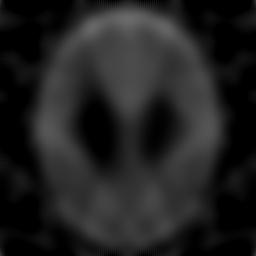
\includegraphics[width=4.5cm]{assets/01}
\caption{\small p=0.1, 10条线}%图片的名称
\label{fig: Figure1}
\end{minipage} 
\hfill
\begin{minipage}[t]{0.4\linewidth}
\centering

\includegraphics[width=4.5cm]{assets/05}
\caption{\small p=0.5, 10条线}%图片的名称
\label{fig: Figure2}
\end{minipage}
\begin{minipage}[t]{0.4\linewidth}%并排放两张图片,每张占行的0.4,下同 
\centering     %插入的图片居中表示
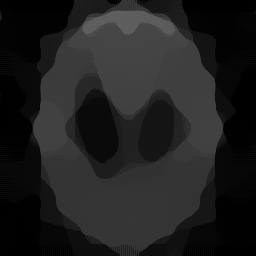
\includegraphics[width=4.5cm]{assets/08}
\caption{\small p=0.8, 10条线}%图片的名称
\label{fig: Figure3}
\end{minipage} 
\hfill
\begin{minipage}[t]{0.4\linewidth}
\centering
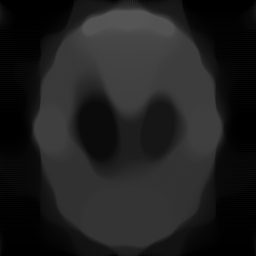
\includegraphics[width=4.5cm]{assets/10}
\caption{\small p=1.0, 10条线}%图片的名称
\label{fig: Figure4}
\end{minipage}
\end{figure}

\subsection{30条线}
为了验证我们的算法确实在极小化TV的$l_p$-norm, 我们增了采样数,为30条线,见图\ref{fig: Figure5}、\ref{fig: Figure6}、\ref{fig: Figure7}、\ref{fig: Figure8}。可以看到效果相比10条线的采样,有很大的提升。

\begin{figure}[H]
\begin{minipage}[t]{0.4\linewidth}%并排放两张图片,每张占行的0.4,下同 
\centering     %插入的图片居中表示
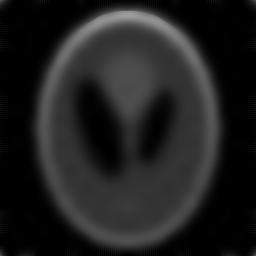
\includegraphics[width=4.5cm]{assets/01-30}
\caption{\small p=0.1, 30条线}%图片的名称
\label{fig: Figure5}
\end{minipage} 
\hfill
\begin{minipage}[t]{0.4\linewidth}
\centering
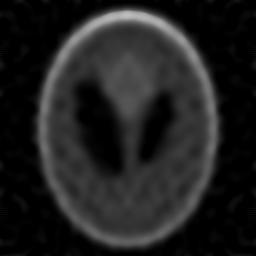
\includegraphics[width=4.5cm]{assets/05-30}
\caption{\small p=0.5, 30条线}%图片的名称
\label{fig: Figure6}
\end{minipage}
\begin{minipage}[t]{0.4\linewidth}%并排放两张图片,每张占行的0.4,下同 
\centering     %插入的图片居中表示
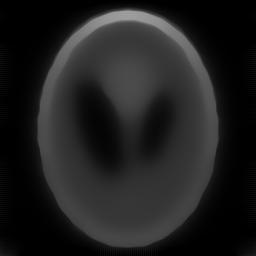
\includegraphics[width=4.5cm]{assets/08-30}
\caption{\small p=0.8, 30条线}%图片的名称
\label{fig: Figure7}
\end{minipage} 
\hfill
\begin{minipage}[t]{0.4\linewidth}
\centering
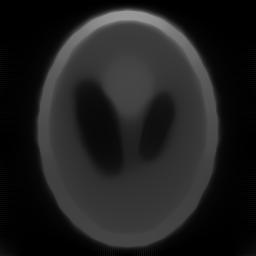
\includegraphics[width=4.5cm]{assets/10-30}
\caption{\small p=1.0, 30条线}%图片的名称
\label{fig: Figure8}
\end{minipage}
\end{figure}

\section{分析}

实验中,正如算法所示,加入$\epsilon$会平滑,以及使得$ (\sqrt{{\nabla u}^2})^{p-2}$有意义,但是算法的初始阶段, $\epsilon$较大,得到的值几乎为0,算法几乎不下降;在$\epsilon$衰减几次后,其不起作用,极小化梯度会使得图像尽可能的平滑(去噪声)。但是,我们没能很好地控制$\epsilon$,造成图像的过度平滑。

\section{代码}

\begin{lstlisting}[language={[ANSI]C},title={homwork.m}]  
clear;clc;
path(path, './Optimization');
path(path, './Measurements');
path(path, './Data');

% Phantom 
n = 256;
N = n*n;
X = phantom(n);
x = X(:);
% l-p norm
epsilon = 10;
factor = 10;
p = 1.0;

% number of radial lines in the Fourier domain
L = 30;

% Fourier samples we are given
[M,Mh,mh,mhi] = LineMask(L,n);
OMEGA = mhi;
A = @(z) A_fhp(z, OMEGA);
At = @(z) At_fhp(z, OMEGA, n);

% measurements
y = A(x);

% min l2 reconstruction (backprojection)
xbp = At(y);
Xbp = reshape(xbp,n,n);

% recovery
tic
[gx, gy] = gradient(X);
tvI = sum(sum(sqrt(gx.^2 + gy.^2)));
fprintf('Original TV = %8.3f\n', tvI);

un = Xbp;
i = 0;
step = 0.01;
dis = 1000;
while true
   i = i + 1;
   [gx, gy] = gradient(un);
   p_norm = sum(sum(power(sqrt(gx.^2 + gy.^2 ), p)));
   
   coef = power(sqrt(gx.^2 + gy.^2 + epsilon^2), p-2); 
   tvU_x = coef .* gx;
   tvU_y = coef .* gy;
   
   dn = -divergence(tvU_x, tvU_y);
   j = 0;
   if mod(i, 100) == 0
       for t = 1e-1: -1e-3 : 1e-4
           j = j + 1;
           u_next = un - t*dn;
           y_next = A(u_next(:));
           if abs(norm(y_next) - norm(y)) < sqrt(epsilon)/100
               break;
           end
       end
       step = t;
   end
   un = un - step*dn;
   [gx, gy] = gradient(un);
   p_norm_next = sum(sum(power(sqrt(gx.^2 + gy.^2 ), p)));
   tol = max(max(un-X));
   if max(max(un-X)) < dis
       dis = tol;
       imwrite(un,['figure/best.jpg']);
   end
   if mod(i, 100) == 0
        fprintf('i=%i, j=%i, rate=%.3f \n', i, j, p_norm_next/p_norm);
   end
   if p_norm_next < p_norm * 0.95 || mod(i, 300) == 0
        fprintf('shrink \n');
        epsilon = epsilon / factor;
        imwrite(un,['figure/', int2str(i), '.jpg']);
   end
   if i > 2000
       break;
   end
end
toc
Xtv = un;
figure();
subplot(1, 3, 1);
imshow(X);
subplot(1, 3, 2);
imshow(Xbp);
subplot(1, 3, 3);
imshow(Xtv);
\end{lstlisting}  

 \begin{thebibliography}{99}
 \bibitem{pa}Rick Chartrand, "Exact reconstructions of sparse signals via nonconvex minimization," IEEE Signal Processing Letters, vol. 14, pp. 707–710, 2007
 \end{thebibliography}
 
\end{document}